\section{Laboratory work implementation}

\subsection{Tasks and Points}

\begin{itemize}
	\item Normal Level 
	\begin{itemize}
		\item Implementeaza un simplu ceas sau stopwatch
	\end{itemize}
\end{itemize}

\subsection{Analiza lucrarii de laborator}

Am dezvoltat o aplicatie Android in IDE-ul AndroidStudio, proiectul construit pe un empty activity.
Activity MainActivity este legat cu layout-ul actity care contine partea grafica ferestrei si arata astfel:

\begin{center}
\includegraphics[width=0.5\linewidth]{"stop 001"}
\end{center}


Aceasta continte 3 Layout-uri verticale.Primul pentru afisarea timerului.Al 2 Layout lam folosit pentru fixarea timpului curent fara oprirea stopwatch-ului.Iar al 3 Layout lam utilizat pentru realizarea a 3 butoane.



Aici putem observa aceste Layout-uri si cum a fost implementat interfata aplicatiei.

\begin{center}
\includegraphics[width=0.7\linewidth]{"stop 003"}
\end{center}

Interfata aplciatiei o realizam cu ajutorul Paletei de intrumente care contine o gama larga


\begin{center}
\includegraphics[width=0.4\linewidth, height=0.4\textheight]{"stop 005"}
\end{center}

Toate butoanele,textele,afisarea,layouturile le putem cu usurinta de modificat/editat Inserand oricare din aceste obiecte observam ca apare o paleta "Properties" care ne ajuta aceasta sa o facem

\begin{center}
\includegraphics[width=0.7\linewidth]{"stop 004"}
\end{center}


Asa arata structura proiectului:

\begin{center}
\includegraphics[width=0.5\linewidth, height=0.3\textheight]{"stop 002"}
\end{center}



Android Studio contine emulator pentru android cu o multime de modele de telefoane cu diferite versiuni de android.Totul se realizeaza cu ajutorul ADM(Android device manager)
Am utilizat ca device NExus S cu android 5.0.
Observam ca stopwatch-ul lucreaza fine
\begin{center}
\includegraphics[width=0.4\linewidth, height=0.4\textheight]{"stop 008"}
\end{center}

Am instalat aceasta aplicatie pe telefonul propriu pentru a o incerca in practica.
Toate 3 butoane implementate lucreaza adecvat conform instructiunilor pe care trebuie sa le efectueze,oarecare baguri nu sau intalnit
\begin{center}
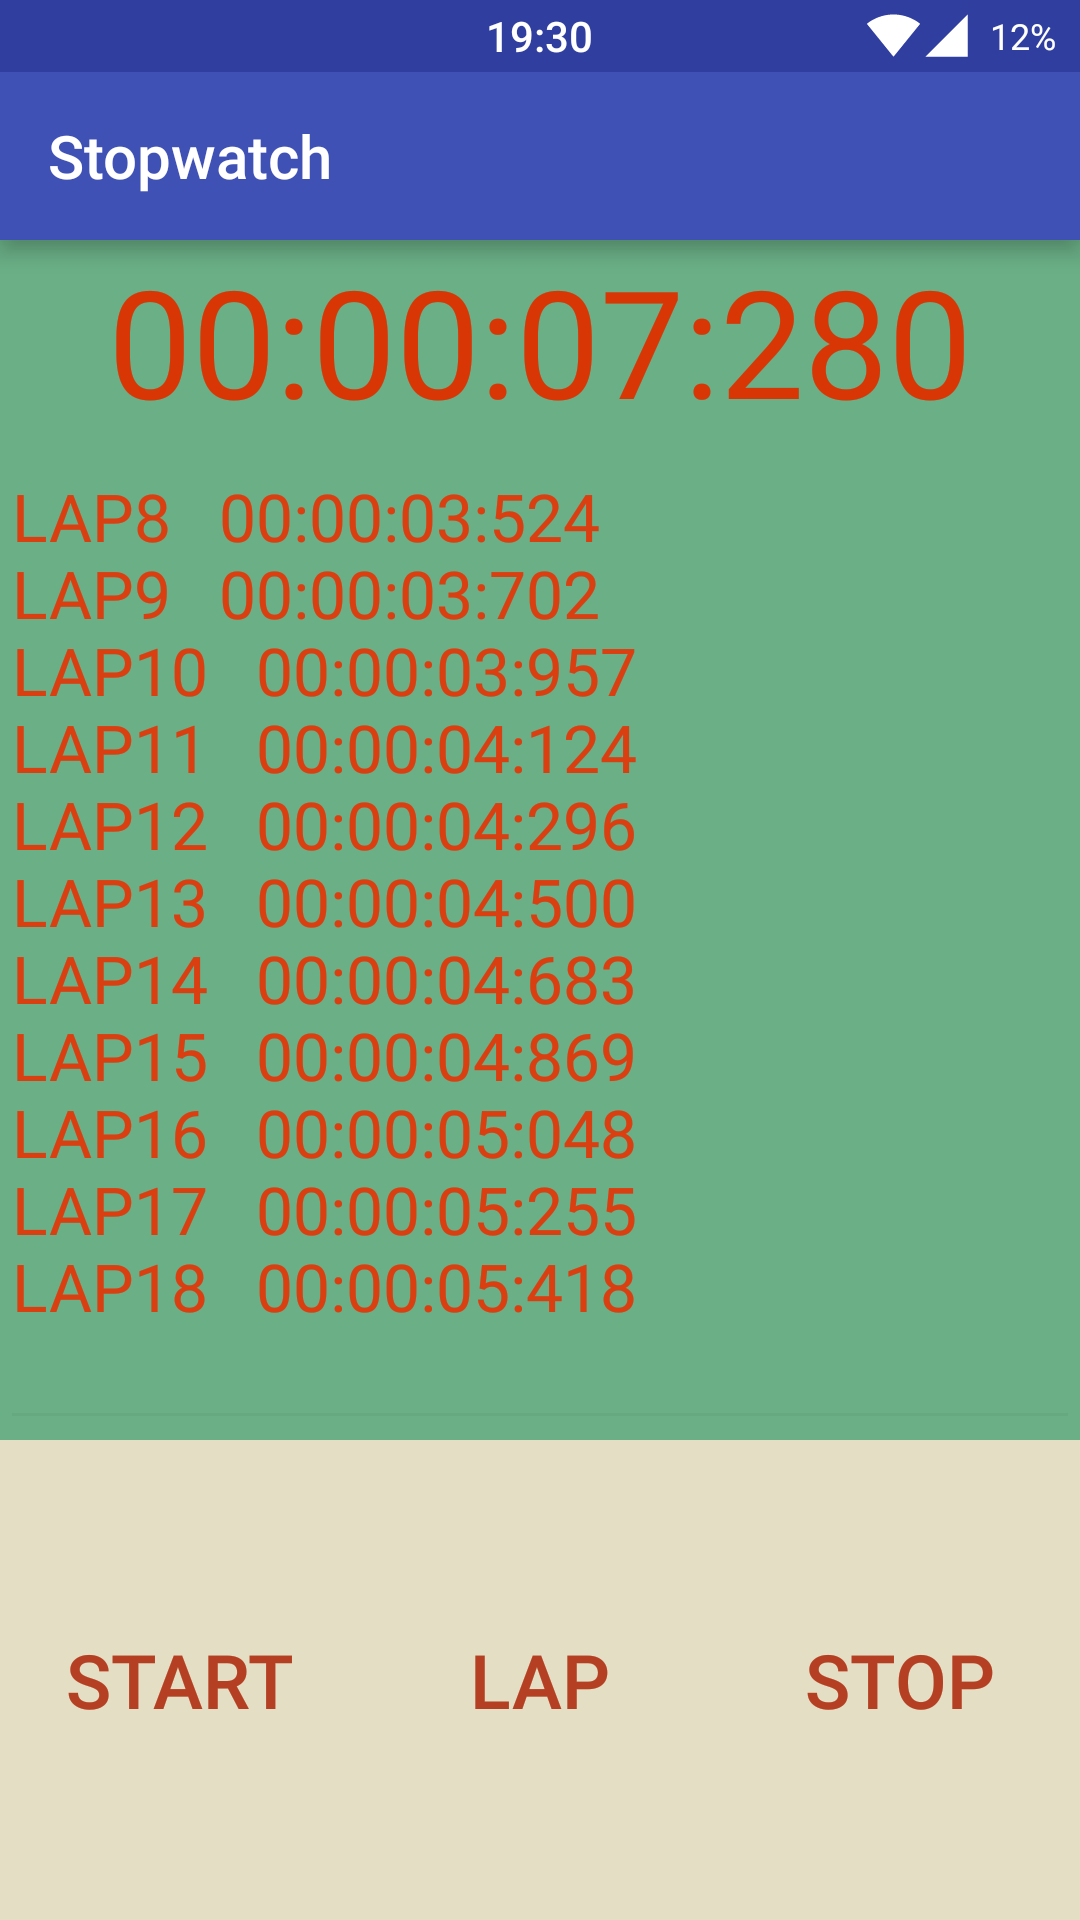
\includegraphics[width=0.4\linewidth, height=0.4\textheight]{Screenshot_20160420-193056}
\end{center}




\clearpage



